
به منظور بررسی کارآیی روش‌های به کار گرفته شده نیاز است تا آن ها را در محیط های مختلفی آزمایش کنیم. اصلی ترین بستری که نیاز است کارآیی مناسبی در آن وجود داشته باشد، محیط واقعی است یعنی الگوریتم‌های مورد بررسی بر گوشی‌های تلفن همراه و محیط سرور پیاده سازی شوند و تشخیص‌ها به خوبی انجام شده ، هشدارها صادر شوند. اما از آنجایی که هزینه‌های مالی و معنوی این کار برای بررسی اولیه الگوریتم زیاد است، نیاز است تا این روش‌ها بر روی دادگان شبیه‌سازی شده و دادگان واقعی گذشته اعمال شود.


\subsection{پیاده‌سازی عملی سیستم}
\todo{بخش پیاده سازی عملی }

\subsection{ استفاده از شبیه‌ساز }
همان‌طور که به میان آمد، برای بهینه کردن پارامترهای الگوریتم ها نیاز است الگوریتم‌ها را محیط هایی ساده پیاده‌سازی کرده و کارآیی آن‌ها را بیشینه کنیم. به همین منظور برای این پژوهش شبیه‌سازی طراحی شده‌است.

 \begin{figure}[H]
	 	\centering
	 	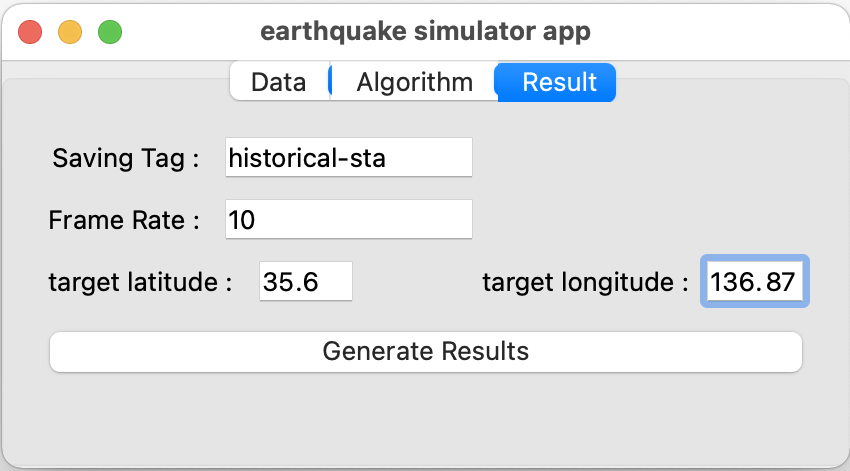
\includegraphics[width=1\textwidth]
	 	{images/simulator.png}
	 	\caption{تصویر فضای شبیه‌ساز}
	 	\label{fig:simulator}
 \end{figure}
 
 این شبیه‌ساز با کمک کتابخانه
\lr{PyQt5}
و با زبان برنامه نویسی پایتون
\LTRfootnote{Python}
 نوشته شده‌است.
 
 
 این شبیه‌ساز در سه گام اطلاعات مورد نیاز را دریافت می‌کند و نتیجه را تولید می‌کند. گام اول، بخش داده 
 \LTRfootnote{Data}
 است . در این بخش دادگان مورد نیاز برای شبیه‌سازی انتخاب می‌شود. گام بعدی، الگوریتم
 \LTRfootnote{Algorithm}
 است. در این گام الگوریتم تخمین مکان لرزش  انتخاب می‌شود. در انتها نیز پارامتر های تولید خروجی در گام نتیجه
 \LTRfootnote{Result}
 تنظیم می‌شود.
 
 
 دو الگوریتم اصلی در شبیه‌ساز قابل انتخاب است. الگوریتم تشخیص مکان بر اساس زمان رسیدن موج و الگوریتم تشخیص بر اساس بیشینه شتاب دریافتی. این الگوریتم ها در بخش بعدی بیشتر توضیح داده شده اند.
 \todo{\lr{link to algorithm section}}
 
 همچنین برای فراهم کردن داده از چند منبع مختلف استفاده شده‌است. منبع اول، استفاده از داده‌های ثبت شده در شبکه‌های لرزه‌نگاری 
\lr{K-NET , KiK-NET}
 است. منبع بعدی، تولید دیتا بر اساس مدل های ساده شده‌ی لرزش زمین است. 
\todo{\lr{link to data import section}}



\subsubsection{دادگان در شبیه‌ساز}
همانطور که در بخش قبل توضیح داده‌شد، به طور کلی از دو منبع برای تولید دیتا بهره جسته‌ایم: دادگان واقعی و دادگان تولید شده به کمک مدل ساده شده‌ی زمین. در این قسمت می‌خواهیم به جزئیات این دو منبع تولید دیتا بپردازیم.
 
\textbf{منبع اول}
 ، استفاده از دادگان شبکه‌های لرزه‌نگاری ژاپن است. اطلاعات دو شبکه‌ی 
\lr{K-NET \LTRfootnote{Kyoshin Network} , KiK-NET\LTRfootnote{Kiban Kyoshin Network}}
به صورت آزاد در سایت رسمی آن
\LTRfootnote{https://www.kyoshin.bosai.go.jp/}
 موجود است.
  \begin{figure}[H]
	 	\centering
	 	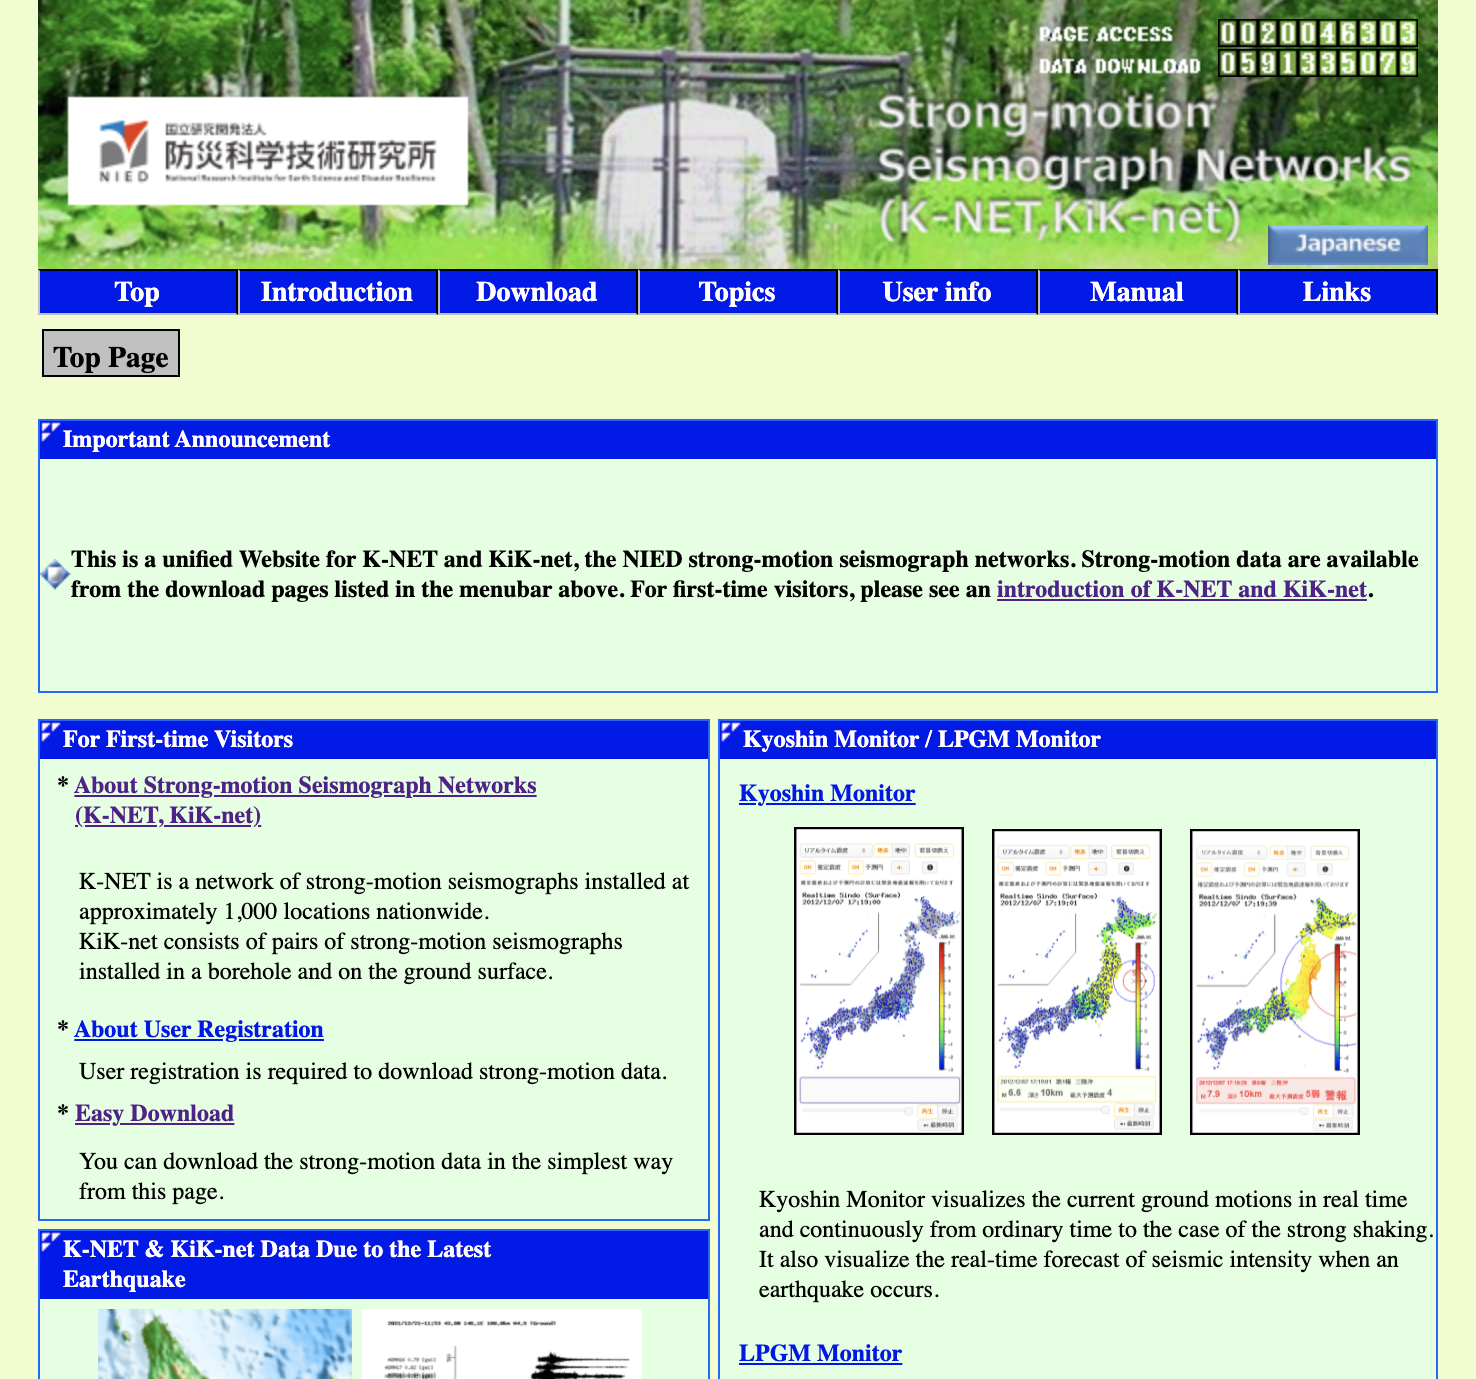
\includegraphics[width=1\textwidth]
	 	{images/japan-website.png}
	 	\caption{صفحه اینترنتی شبکه‌های لرزه‌نگاری ژاپن
	 	}
	 	\label{fig:japan-website}
 \end{figure}
 
 شبکه لرزه‌نگاریK-NET یک شبکه سراسری لرزه‌نگاری در کشور ژاپن است. این شبکه شامل بیش از ۱۰۰۰ دستگاه جمع‌آوری داده است. این دستگاه‌ها به صورت یکنواخت گسترده شده‌اند. این شبکه از سال ۱۹۹۶ تحت نظر موسسه ملی تحقیقات علوم زمین و مقاومت در برابر بلایا
\LTRfootnote{National Research Institute for Earth Science and Disaster Resilience (NIED)}
فعالیت می‌کند.\cite{japan-seismograph-network}

شبکه لرزه‌نگاری KIK-NET نیز شامل ۷۰۰ ایستگاه در سرتاسر ژاپن است. در این ایستگاه‌ها یک جفت لرزه‌نگار با حساسیت بالا
\LTRfootnote{Hi-net}
 در چاه گمانه
\LTRfootnote{borehole}
نصب شده‌است. یکی از این دو حسگر بر سطح زمین و دیگری در عمق صد متری سطح قرار می‌گیرد. شبکه‌ی KIK-NET تحت برنامه‌ی بررسی و رصد بنیادی برای تحقیقات زلزله تحت نظر موسسه ملی تحقیقات علوم زمین و مقاومت در برابر بلایا ساخته شده‌است.  دادگان ثبت شده در این دو شبکه به سرعت به مرکز مدیریت دادگان NIED منتقل و ذخیره می‌شود.  

دادگان قرار داده شده در این سایت از استاندارد خاص خود پیروی می‌کند
\lr{K-NET ASCII format}
. در این قالب اطلاعات زیر به اشتراک گذاشته شده‌است:

\begin{itemize}
\item{زمان وقوع لرزش
\LTRfootnote{origin time}
}
\item{طول و عرض جغرافیایی ایستگاه}
\item{ارتفاع ایستگاه}
\item{طول و عرض جغرافیایی مرکز لرزش}
\item{عمق وقوع لرزش}
\item{شدت وقوع لرزش}
\item{زمان اولین نمونه}
\item{نرخ نمونه‌برداری}
\item{ضریب مقیاس ( ضریبی که برای تبدیل به مقیاس گالیله
\LTRfootnote{$1\ gal = 1\ cm/s^{2}$}
 نیاز است)}
\item{دادگان خام ضبط شده در ایستگاه}
\end{itemize}

این سامانه سالیانه هزاران لرزش در محدوده‌ی ژاپن را ثبت و ذخیره می‌کند. برای این پژوهش دادگان ایستگاه‌هایی با مشخصات زیر استفاده شده‌اند:
\begin{itemize}
	\item{عرض جغرافیایی بین ۳۵ تا۳۶.۴ درجه}
	\item{طول جغرافیایی بین ۱۳۶.۴ تا ۱۴۰.۳۱ درجه}
	\item{شدت لرزش بیشتر از ۴.۵ ریشتر}
	\item{فاصله ایستگاه‌ها کمتر از ۶۰ کیلومتر تا منبع وقوع لرزش}
\end{itemize}

  \begin{figure}[H]
	 	\centering
	 	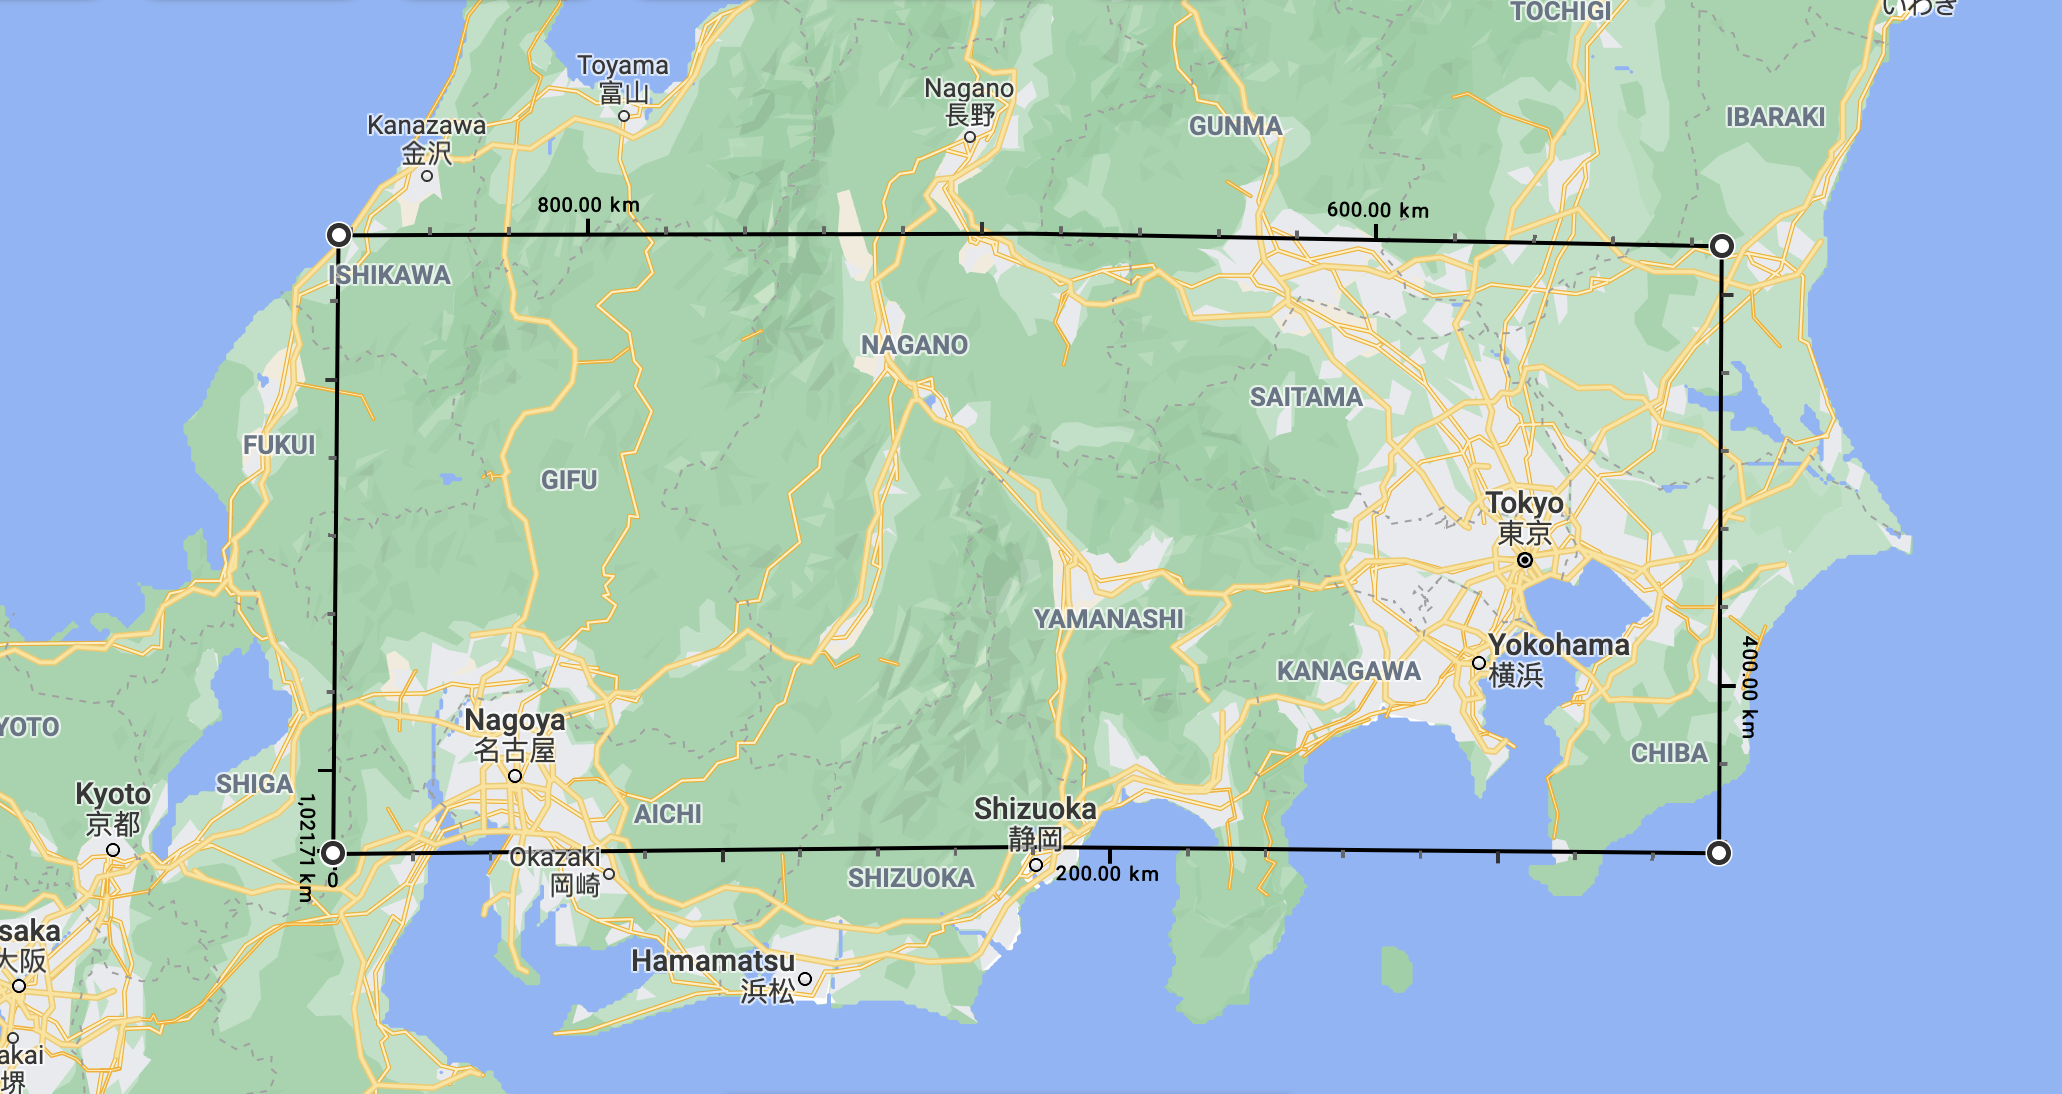
\includegraphics[width=1\textwidth]
	 	{images/japan-area.png}
	 	\caption{محدوده‌ی ایستگاه‌های استفاده شده}
	 	\label{fig:japan-area}
 \end{figure}
 
محدوده‌ی انتخاب شده در تصویر \ref{fig:japan-area}  نشان داده شده‌است.


همان‌طور که گفته شد، منبع اول دادگان، استفاده از دادگان واقعی ثبت شده در شبکه لرزه‌نگاری کشور ژاپن است. 
\textbf{منبع دوم}
دادگان در این پژوهش دادگان تولید شده به کمک مدل ساده شده‌ی زمین است. 

 یک مدل ساده شده برای تولید داده به صورت زیر است:
\begin{equation}
	\label{eq:sim-exp-eq}
	attenuation = e^{-\ c \ d}
\end{equation}
\todo{مرجع برای این رابطه توانی اگر پیدا بشه بیاد خیلی خوبه}
که d فاصله بین مرکز و ایستگاه است و ضریب c ضریب تضعیف است. برای اینکه شبیه سازی به صورت واقعی‌تری انجام شود، ضرایب تضعیف در نقاط مختلف را متفاوت فرض کردم. همانطور که در 
\ref{fig:attenuation-map}
آمده است، فضا به صورت خانه‌های کوچک فرض شده است و مقدار تضعیف در هر خانه متفاوت با بقیه است.

 \begin{figure}[H]
	 	\centering
	 	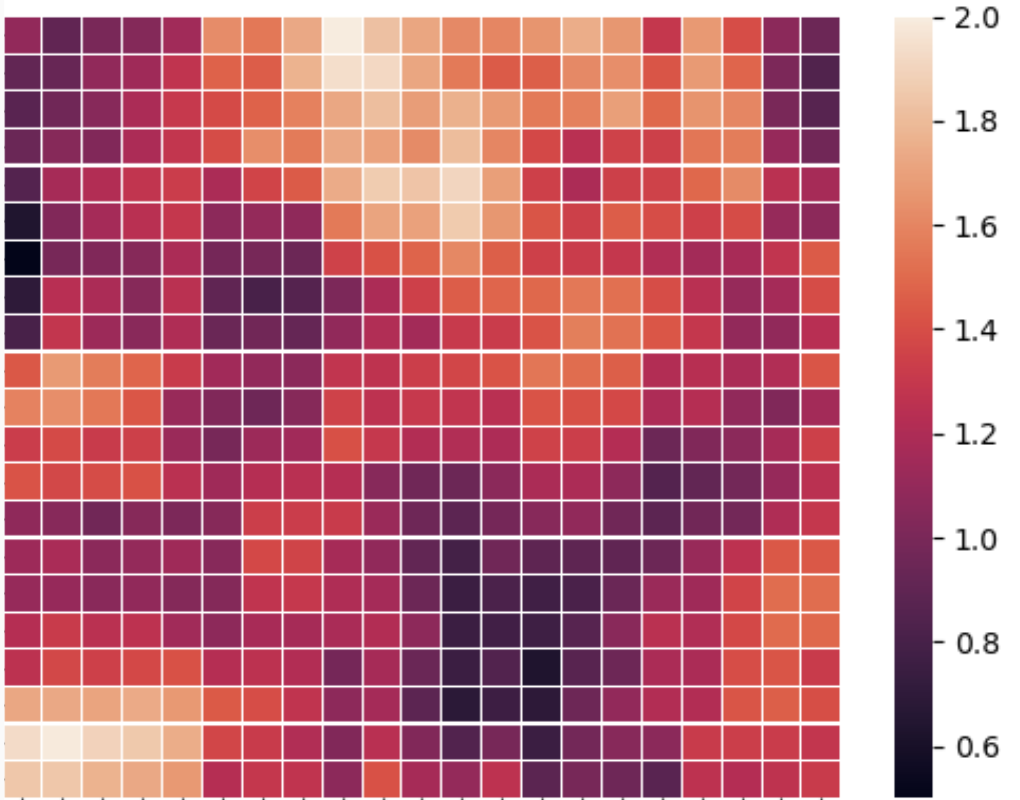
\includegraphics[width=1\textwidth]
	 	{images/attenuation-map.png}
	 	\caption{نقشه تضعیف در نقاط مختلف شبیه‌ساز}
	 	\label{fig:attenuation-map}
 \end{figure}
 
 باتوجه به اینکه ضریب تضعیف در نقاط مختلف متفاوت است، در هر خانه تضعیف متفاوتی اتفاق می‌افتد و رابطه 
 \ref{eq:sim-exp-eq}
 به صورت زیر بازنویسی و اجرا می‌شود:
 
 \begin{equation}
	\label{eq:sim-exp-end-eq}
	attenuation = e^{-\Sigma_{i=1}^{n} c_{i}d_{i}}
%	\Delta t = \frac{\Sigma_{i=1}^{n}d_{i}}{v} 
\end{equation}

\begin{equation}
	\label{eq:sim-exp-time}
	\Delta t = \frac{\Sigma_{i=1}^{n}d_{i}}{v} 
\end{equation}
 
 علاوه بر تضعیف، باتوجه به فاصله‌ی ایستگاه و منبع یک تفاوت زمانی نیز وجود دارد که این تفاوت با کمک رابطه
 \ref{eq:sim-exp-time}
 محاسبه می‌شود. در این رابطه پارامتر v  با یک مقدار ثابت تعیین می‌شود. در انتها برای تولید یک سیگنال تضعیف شده در مکان‌های دیگر، یک سیگنال مرجع به این تولید کننده تزریق می‌شود و پس از اعمال تضعیف و تاخیر سیگنال دریافت شده، سیگنال خروجی بازسازی می‌شود.
\begin{figure}[H]
	 	\centering
	 	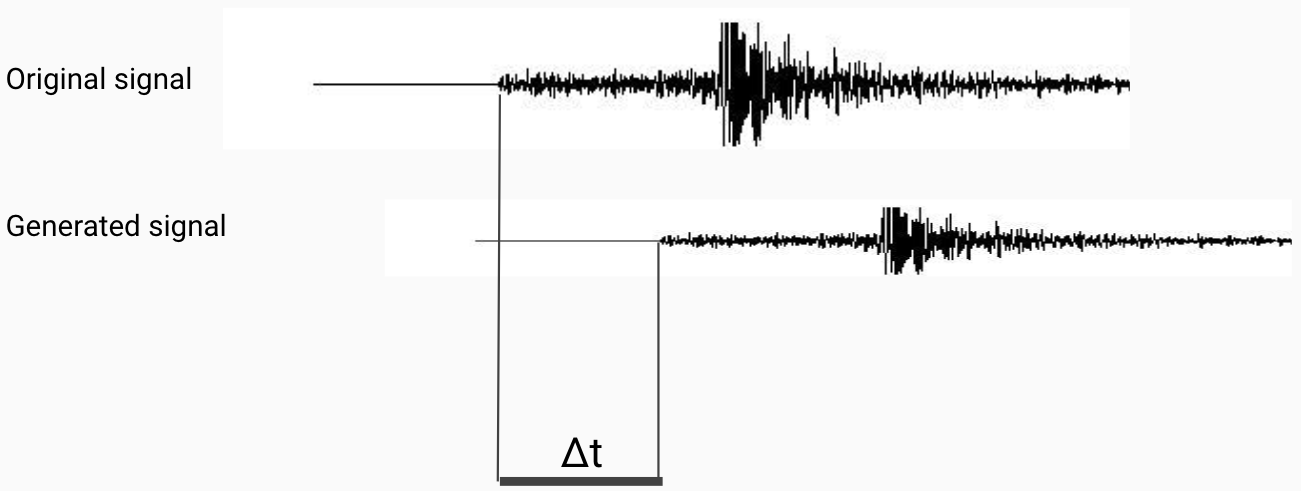
\includegraphics[width=1\textwidth]
	 	{images/signal-generation.png}
	 	\caption{شماتیک تولید سیگنال خروجی}
	 	\label{fig:signal-generation}
\end{figure} 
 
همان‌گونه که در تصویر 
\ref{fig:signal-generation}
دیده می‌شود، سیگنال خروجی حاصل تغییر مقیاس و شیفت زمانی محاسبه شده بر روی سیگنال مبدا است.
 
 شیوه دیگر تولید سیگنال شبیه‌سازی خروجی نسبت به سیگنال مبدا استفاده از رابطه‌ی تضعیف 
\ref{eq:attenuation-geo-formula}
است
\cite{Denham_Small_1971} 
 .
\begin{equation}
	\label{eq:attenuation-geo-formula}
	\log Y = b_{1}+b_{2}M+b_{3}\log R
\end{equation}
 در این شیوه نیز پس از اینکه پارامتر های تضعیف
$b_{i}$
تعیین شدند، تاخیر و میزان تضعیف در هر نقطه مشخص می‌شود و به مانند تصویر
\ref{fig:signal-generation}
سیگنال خروجی تولید می‌شود. 
 
 
 
 
 
 
 
 
 
 
 
 